% !TeX spellcheck = <none>
\documentclass[brudnopis]{xmgr}
% Jeśli nowe rozdziały mają się zaczynać na stronach
% nieparzystych:
%\documentclass[openright]{xmgr}

\usepackage{epigraph}
\usepackage{url}
\usepackage{float}

\defaultfontfeatures{Scale=MatchLowercase}
\setmainfont[Numbers=OldStyle,Ligatures=TeX]{Minion Pro}
\setsansfont[Numbers=OldStyle,Ligatures=TeX]{Myriad Pro}
% for fontspec version < 2.0
%\setmainfont[Numbers=OldStyle,Mapping=tex-text]{Minion Pro}
\setsansfont[Numbers=OldStyle,Mapping=tex-text]{Myriad Pro}
%\setmonofont[Scale=0.75]{Monaco}

% Code listing
%\usepackage{bera}% optional: just to have a nice mono-spaced font
\usepackage{listings}
\usepackage{xcolor}

\colorlet{punct}{red!60!black}
\definecolor{background}{HTML}{EEEEEE}
\definecolor{delim}{RGB}{20,105,176}
\colorlet{numb}{magenta!60!black}

\lstdefinelanguage{json}{
    basicstyle=\normalfont\ttfamily,
    numbers=left,
    numberstyle=\scriptsize,
    stepnumber=1,
    numbersep=8pt,
    showstringspaces=false,
    breaklines=true,
    frame=lines,
    backgroundcolor=\color{background},
    literate=
        *{0}{{{\color{numb}0}}}{1}
        {1}{{{\color{numb}1}}}{1}
        {2}{{{\color{numb}2}}}{1}
        {3}{{{\color{numb}3}}}{1}
        {4}{{{\color{numb}4}}}{1}
        {5}{{{\color{numb}5}}}{1}
        {6}{{{\color{numb}6}}}{1}
        {7}{{{\color{numb}7}}}{1}
        {8}{{{\color{numb}8}}}{1}
        {9}{{{\color{numb}9}}}{1}
        {:}{{{\color{punct}{:}}}}{1}
        {,}{{{\color{punct}{,}}}}{1}
        {\{}{{{\color{delim}{\{}}}}{1}
        {\}}{{{\color{delim}{\}}}}}{1}
        {[}{{{\color{delim}{[}}}}{1}
        {]}{{{\color{delim}{]}}}}{1},
}

% END Code listing

% Opcjonalnie identyfikator dokumentu
% drukowany tylko z włączoną opcją 'brudnopis':
\wersja   {wersja wstępna [\ymdtoday]}

\author   {Piotr Lewandowski}
\nralbumu {215575}
\email    {poczta@piotrl.net}

\title    {Analiza wpływu nawyków muzycznych na aktywności wykonywane przy komputerze}
\date     {2017}
\miejsce  {Gdańsk}

\opiekun  {dr W. Bzyl}

% dodatkowe polecenia
%\renewcommand{\filename}[1]{\texttt{#1}}
%\definecolor{stress}{cmyk}{0,1,0.13,0} % RubineRed
%\definecolor{topic}{cmyk}{0.98,0.13,0,0.43} % MidnightBlue

\begin{document}

% streszczenie
\begin{abstract}
    W ramach pracy magisterskiej napisano aplikację internetową,
    wdrożoną w chmurze Digital Ocean pod adresem http://tbd.digitalocean.com/
    z przygotowanymi danymi testowymi pod kontem (user: test, login: test).

    Aplikacja umożliwia agregację danych użytkownika z dwóch serwisów,
    RescueTime — lista aktywności oraz
    Last.fm — lista odsłuchiwanych utworów.
    Pobrane dane są połączone na wspólnej osi czasu i wizualizowane pod różnymi względami za pomocą wykresów oraz tabel.

    Mechanizm agregacji napisany jest w języku Java i frameworku Spring,
    dane przechowywane są w bazie danych PostgreSQL,
    a warstwa wizualna została stworzona w JavaScript
    z użyciem biblioteki generującej wykresy — C3.js
    oraz frameworka Material Design.

    Kod znajduje się w prywatnym repozytorium GIT (pod adresem \url{https://github.com/piotrl/master-thesis}),
    pytania o dostęp lub o pracę można kierować na mail: poczta@piotrl.net.
\end{abstract}

% słowa kluczowe
\keywords{
    Aggregation,
    Data Integration,
    Data Visualisation,
    PostgreSQL,
    JavaScript,
    Java
}

% tytuł i spis treści
\maketitle

% wstęp
\introduction

\epigraph{Without deviation from the norm, progress is not possible}{\textit{Frank Zappa}}

[Work in progress]

Podczas pracy często słucham muzyki, by się odciąć od zewnętrznych dźwięków oraz odpowiednio nastroić.
Spotyka się na artykuły twierdzące, że odpowiednio dobrana muzyka wpływa na lepszą koncentrację.
Popularnym przykładem jest wystąpienie Willa Henshalla na konferencji TEDx,
którą w momencie pisania pracy obejrzano ponad 400 tysięcy razy:

Jednym z pytań w corocznej sondzie serwisu StackOverflow jest pytanie o muzyczne preferencje podczas programowania.
Na to pytanie odpowiedziało ponad 36 tysięcy osób \cite{stackoverflow:survey2017}.

\begin{figure}
  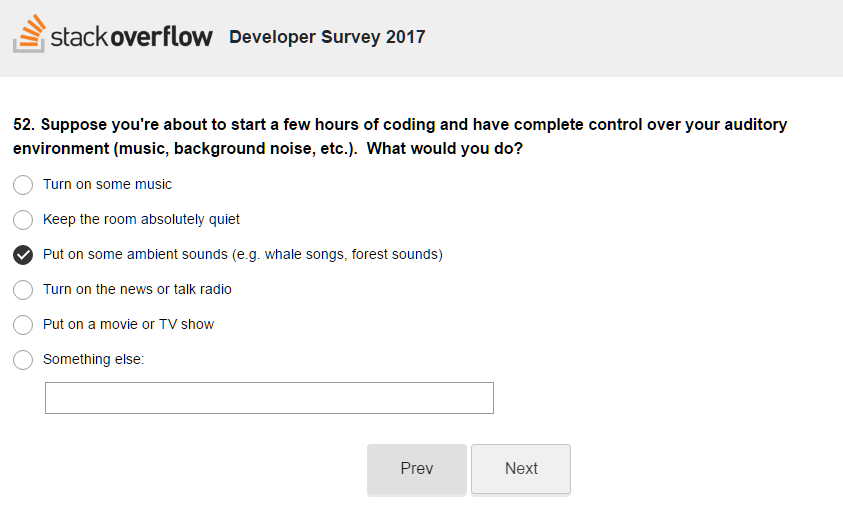
\includegraphics[width=\linewidth]{fig/stack_overflow_music.png}
  \caption{Pytanie o preferncje muzyczne na StackOverflow}
  \label{fig:Pytanie o preferncje muzyczne na StackOverflow}
\end{figure}

\chapter{Import danych}

    \section{Wybór dostawców danych}

    Podstawą działania aplikacji są dane z komputera użytkownika,
    lista aktywności wykonywanych w danej jednostce czasu oraz odsłuchiwana muzyka.
    Aby zdobyć te dane, postanowiłem nie pisać programu śledzącego procesy (daemon),
    lecz skorzystać z istniejących serwisów, z których użytkownicy mogli już korzystać.

    Przy wyborze rozwiązania zależało mi na tym, by serwisy były już dłuższy czas na rynku
    oraz udostępniały archiwalne dane za pomocą publicznego API.
    Dzięki temu nie ma potrzeby oczekiwania na zbudowanie zioru danych do analizy po rejestracji nowego użytkowniku,
    od razu można przeanalizować dane z okresu sprzed rejestracji.

    Zdecydowałem się skorzystać z dwóch dobrze znanych mi serwisów - RescueTime oraz last.fm,
    oba serwisy są najpopularniejsze w swojej klasie oraz dostarczają publiczne API dla danych użytkownika.

        \section*{RescueTime}

%        \begin{figure}
%          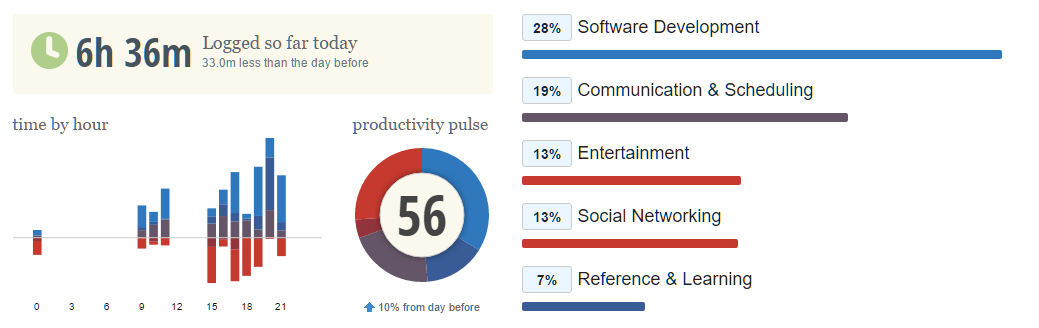
\includegraphics[width=\linewidth]{fig/rescuetime-daily-dashboard.png}
%          \caption{Codzienny raport aktywności RescueTime}
%          \label{fig:RescueTime}
%        \end{figure}

        RescueTime to program, który loguje aktualnie otwarte okna
        i raz na minutę wysyła te dane do serwisu internetowego RescueTime.com.
        Podstawową cechą tego serwisu jest automatyczne kategoryzowanie aktywności oraz ustawienie produktywności w 5 punktowej skali:
        „Bardzo produktywny”, „Produktywny”, „Neutralny”, „Rozpraszający” i „Bardzo rozpraszający”.

        Serwis uczy się doasowywać aktywności do kategorii na podstawie wcześniejszych oznaczeć użytkowników.
        Dla przykładu odtwarzacz wideo VLC jest przypisany do kategorii „Entertainment” ze statusem „Bardzo rozpraszający”,
        natomiast przeglądanie plików programem Windows Explorer jest w kategorii „Utilities” ze statusem „Neutralny”.

        Dzięki temu jesteśmy w stanie obliczyć nasz codzienny współczynnik produktywności,
        sumując czas spędzony na aktywnościach z każdej kategorii.

        \begin{table}[]
        \centering
        \begin{tabular}{lll}
        \hline
        \multicolumn{1}{l|}{Aktywność} & \multicolumn{1}{l|}{Kategoria} & Produktywność \\ \hline
        idea64                         & Software Development           & +2            \\
        NotePad++                      & Software Development           & +2            \\
        postgresql.org                 & Reference \& Learning          & 0             \\
        twitter.com                    & Social Networking              & -1            \\
        analytics.twitter.com          & Social Networking              & -2            \\
        youtube.com                    & Entertainment                  & -2            \\
        outlook.office.com             & Communication \& Scheduling    & 0             \\
        wunderlist                     & Business                       & +2
        \end{tabular}
        \caption{
            Lista przykładowych aktywności wraz z ich kategoriami. Skala produktywności od +2 do -2
            \newline Źródło: Opracowanie własne.
        }
        \label{RescueTime - lista przykładowych aktywności}
        \end{table}

            Program jest w stanie rozpoznać nie tylko tytuły aktualnie otwartych okien,
            ale również w przypadku przeglądarki – adresy odwiedzanych stron internetowych,
            jest to bardzo ważne ze względu na dominującą ilość czasu spędzonego w samej przeglądarce.

            Dostęp do informacji użytkownika odbywa się po REST API z tokenem uwierzytelniającym,
            który użytkownik musi wygenerować na stronie RescueTime.com.
            Po poprawnym uwierzytelnieniu, mamy dostęp do danych sprzed 3 miesięcy w formacie JSON.

        \section*{last.fm}

            Last.fm to serwis społecznościowy dla fanów muzyki,
            pomagający odkrywać nowych artystów na podstawie historii użytkownika.

            Wtyczka "last.fm Scrobbler"\cite{lastfm:trackmymusic} integruje się z wieloma odtwarzaczami muzycznymi, np. Spotify.
            Każdy odsłuchany w co najmniej w połowie utwór jest logowany do bazy danych,
            w której na podstawie meta-tagów jest przypisywany do artysty, płyty oraz gatunku muzycznego.

            Last.fm udostępnia szereg metod REST API \cite{lastfm:apidoc},
            dla mnie szczególnie istotne są te związane z odtworzeniami użytkownika oraz szczegółowych informacji o piosenkach i artystach.

            Metoda user.getRecentTracks % TODO

		% identyfikuje swoje dane za pomocą MBID \cite{lastfm:mbid}

        \begin{figure}
          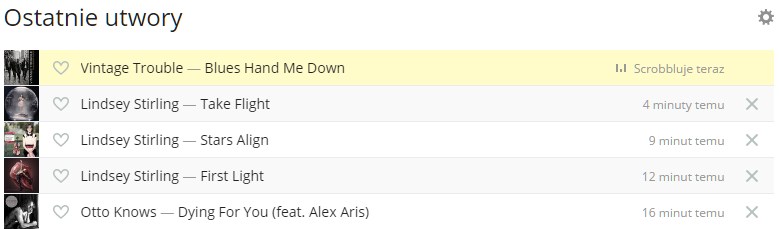
\includegraphics[width=\linewidth]{fig/lastfm-now-listening.png}
          \caption{Raport słuchanej muzyki w last.fm}
          \label{fig:Last.fm}
        \end{figure}

    \section{Mechanizm importu danych}
        Oba z wymienionych serwisów udostępniają część danych, które użytkownik zgromadził na swoim koncie.
        Dostęp ten jest realizowany przez API, po okazaniu odpowiednich tokenów uwierzytelniających, mamy dostęp do danych użytkownika.

        Przed analizą, konieczne jest pobranie danych do własnej bazy danych oraz stworzenie modelu relacji pomiędzy nimi.
        Proces pobierania nazywam agregacją danych lub importem danych i jest on podstawą działania aplikacji,
        ponieważ to w nim zdobywamy interesujące nas informacje wykorzystywane do późniejszych obliczeń.

        Aby aplikacja nie była jednorazowego użytku, wraz z upływem czasu należy dla każdego użytkownika dostarczać
        kolejne porcje danych z zewnętrznych serwisów.
        Rodzi to szereg problemów oraz wyznacza pewne cechy, które napisany mechanizm musi spełniać.

        \subsection*{Niezależność}
            Podczas pobierania danych dla jednego użytkownika może wystąpić błąd, np. poprzez tymczasową niedostępność API,
            nie powinien on wpłynąć na agregacje innych użytkowników, ani na działanie mechanizmu w przyszłości dla tego samego użytkownika.

            Części błędów można się spodziewać, np. lastfm udostępnia do każdej metody API listę błędów które może zwrócić zamiast odpowiedzi.
            Z drugiej strony, mogą wystąpić błędy po naszej stronie - zwłaszcza gdy API nie jest bardzo dobrze udokumentowane
            lub nie mamy zbyt dużego doświadczenia z pracy z nimi, np. podczas mapowania odpowiedzi na obiekty lub przy zapisie danych do bazy.

            Można sobie z tym radzić na kilka sposobów, przechwytując wyjątki podczas wysyłania każdego requestu
            oraz dodatkowy error handler przechwytujący wszystkie wyjątki powstałe podczas budowania modelu i zapisywania danych w bazie.

            Dzięki kilku poziomom przechtywywania wyjątków, mamy możliwość różnicowania o ich krytyczności. 
            Możemy kolejkować nieudane requesty i po kilku minutach ponowić próbę ich wysłania. Jest to skuteczne rozwiązanie gdy API ma sztywny czas sesji po którym następuje wylogowanie.
            RescueTime i last.fm mają autoryzację bezstanową, w pełni polegającej na raz wygenerowanym kluczu - sesja nie jest tu problem, więc zdecydowałem się porzucić pomysł kolejkowania pojedynczych requestów.

            % TODO: Blad w jedenej agregacji nie wplywa na nastepne / kolejnych uzytkownikow

        \subsection*{Ciągłość}

            \begin{figure}
                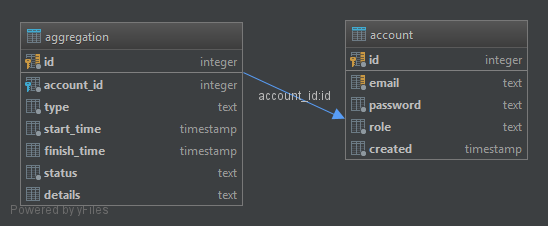
\includegraphics[width=\linewidth]{fig/db-aggregation.png}
                \caption{Schemat relacji aggregation}
                \label{fig:Relacja aggregation}
            \end{figure}
            Celem codzienne uruchamianie procedury i pobranie najnowszych lub brakujących danych do systemu,
            API pozwalają nam na wybranie tylko małego fragmentu danych, istotne jest więc by zacząć import
            od momentu ostatniego poprawnie wczytanego rekordu dla danego użytkownika.

        \subsection*{Powtarzalność}

    \section{Komunikacja z API}

        \subsection*{Specyfika API}
            Przy projektowaniu rozwiązania warto pamiętać o tym, że nie istnieje powszechnie wykorzystywany standard budowania API,
            a każdy dostawca implementuje je w sposób specyficzny dla swojego stystemu i danych jakie udostępnia.

            RescueTime mimo, że co do sekundy loguje start i koniec aktywności,
            jego najwyższa dokładność oferowana użytkownikowi to 5 minut \footnote{TODO: rescuetime:apidoc-precision},
            a w darmowej wersji zezwala na dostęp maksymalnie trzy miesiące wstecz.
            Jest możliwość sterowania formatem odpowiedzi z serwera, CSV lub JSON - jednak JSON	

            \begin{lstlisting}[language=json,firstnumber=1]
{"menu": {
  "id": "file",
  "value": "File",
  "popup": {
    "menuitem": [
      {"value": "New", "onclick": "CreateNewDoc()"},
      {"value": "Open", "onclick": "OpenDoc()"},
      {"value": "Close", "onclick": "CloseDoc()"}
    ]
  }
}}
0123456789
            \end{lstlisting}


        \subsection*{Autoryzacja}
        
        Do każdego requestu należy dodać klucze autoryzujące, które użytkownik musi wygenerować w serwisach Last.fm i RescueTime \cite{rescuetime:apidoc-keymanagment} oraz dodać w ustawieniach aplikacji. Klucze zapisywane są ws tabeli \textit{aggregation\_metadata}.
        
        Last.fm wymaga rejestracji aplikacji, po którym otrzymujesz dwa klucze: sekretny i normalny.
        
        W obu serwisach dostępne jest logowanie za pomocą OAuth, dzięki temu użytkownik nie musi samodzielnie generować kluczy, 
        a jedynie potwierdzić chęć udostępnienia swoich danych w aplikacji. W obecnej wersji applikacji nie używam tego mechanizmu.
        
        \begin{figure}
        	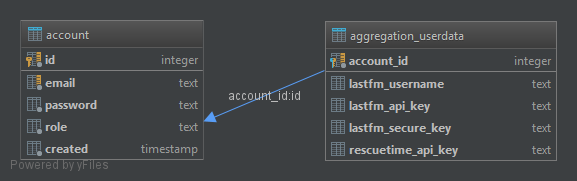
\includegraphics[width=\linewidth]{fig/db-aggregation-metadata.png}
        	\caption{Schemat relacji aggregation\_metadata}
        	\label{fig:}
        \end{figure}

        \subsection*{Niepełne dane}
        API nie gwarantuje istnienia ani poprawności wszystkich informacji.
        Przykładowo last.fm do identyfikacji utworu dostarcza jego MBID oraz pełną nazwę.
        Bezpieczniej jest korzystać z identyfikatora mbid, ponieważ w nazwie mogą występować problematyczne znaki UTF-8 np. w przypadku Chińskich artystów.
        Niekiedy nie jest to możliwe, istnieją bowiem rekordy, dla których identyfikator jest pusty.

        W przypadku RescueTime nie doszukałem się danych, które mógłbym uznać za niepełne.

        \subsection*{Wydajność}
        Dobrze jest kopiować wszystkie powtarzalne informacje do własnej bazy danych,
        dzięki temu możemy ograniczyć ilość żądań do API tylko do nieznanych nam obiektów i zmniejszyć ryzyko wyczerpania limitu requestów.

		Jest to istotna optymalizacja, przy skali tysięcy requestów i średnim czasie requestu wahającym się między 0.5s a 2s,
		robi to różnicę minut.

\chapter{Analiza danych}

	Po pojawieniu się pierwszych danych można zacząć je przeszukiwać i eksperymentalnie łączyć między sobą.
	Zacznę od zobrazowania skali danych, po jakiej się poruszam.
	Zaimportowane dane są z okresu od 31 stycznia do 4 maja 2017 z aktywności wykonywanych na prywatnym laptopie
	oraz od 3 lutego do 4 maja 2017 ze słuchanej muzyki z wielu urządzeń i komputerów.

	W tym 3 miesięcznym okresie wykonałem 34611 akcji, które są przypisane do 1916 programów lub stron internetowych z podziałem na 62 kategorie.
	Łącznie 588 godzin w ciągu 94 dni, średnio 6.2 godziny dziennie.
	Z czego 60.5\% to aktywności oznaczone jako produktywne, a 39.5\% jako rozpraszające lub neutralne.

	W ciągu 91 przeanalizowanych dni przesłuchałem 395 godzin muzyki — średnio 4.3 godziny dziennie.
	Składa się na to 5203 odtworzeń piosenek, z czego 2303 unikalnych wśród 1155 artystów.
	Odsłuchane piosenki były przypisane przez społeczność last.fm do 1185 różnych tagów — najpopularniejsze z nich to: rock, polish, soundtrack
	(przyporządkowane odpowiednio do 543, 423, 347 piosenek).

	Warto już na początku zwrócić uwagę na długość pojedynczych akcji, 38\% ze wszystkich pojedynczych akcji trwało poniżej 10 sekund. % TODO: 19 sekund czy 5? Decyzja.
	Duża część z nich byłą nieskategoryzowana, lub szybkim wyszukiwaniem.
	Natomiast zaledwie 17\% akcji trwało ponad 2 minuty, w tym przypadku częstszą kategorią są rzeczy związane z programowaniem oraz grami.

	    \begin{table}[]
        \centering
        \begin{tabular}{|l|l|l|}
            \hline
            Kategoria                           & Ilość zadań (x)   & \%      \\ \hline
            \multicolumn{2}{|c|}{Zadania trwające poniżej 5 sekund} & x / 6784\\ \hline
            Browsers                            & 1040              & 15.3\%  \\ \hline
            General Utilities                   & 755               & 11.1\%  \\ \hline
            GeneralSocial Networking            & 564               & 8.3\%   \\ \hline
            Search                              & 563               & 8.2\%   \\ \hline
            Uncategorized                       & 551               & 8.1\%   \\ \hline
            \multicolumn{2}{|c|}{Zadania trwające ponad 2 minuty}   & x / 5012\\ \hline
            Browsers                            & 1047              & 20.8\%  \\ \hline
            Editing \& IDEs                     & 821               & 16.3\%  \\ \hline
            General Social Networking           & 570               & 11.3\%  \\ \hline
            General Software Development        & 408               & 8.1\%   \\ \hline
            Games                               & 282               & 5.6\%   \\ \hline
        \end{tabular}
        \caption{Lista najpopularniejszych kategorii wśród krótkich zadań poniżej 5 sekund oraz tych powyżej 2 minut}
        \label{Zadania krótkie i długie, które są najpopularniejsze?}
        \end{table}

\section{Opis zebranych danych}

    \begin{figure}
        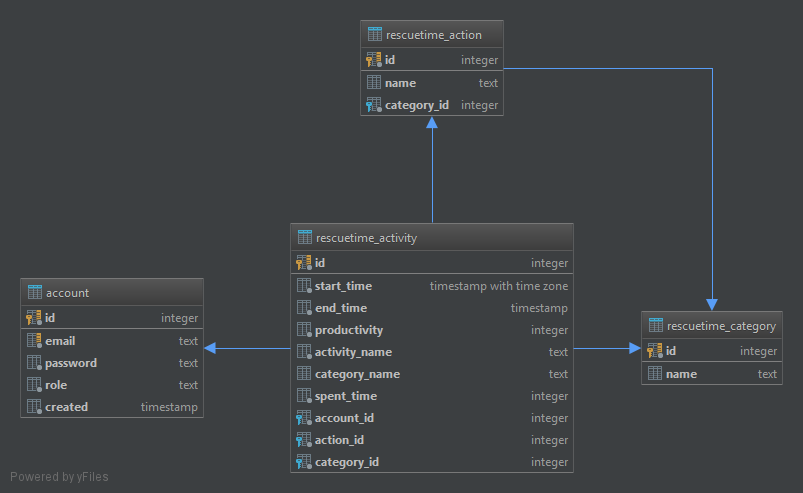
\includegraphics[width=\linewidth]{fig/db-rescuetime-schema.png}
        \caption{Schemat relacji danych o aktywnościach}
        \label{fig:Dane z RescueTime - Schemat relacji}
    \end{figure}

    Najważniejszą tabelą wśród tych powiązanych z aktywnościami jest \verb|rescuetime_activity|,
    to do niej w pierwszej kolejności trafiają dane z API bez żadnej obróbki,
    następnie nazwa akcji oraz kategoria są przyporządkowywane do istniejących rekordów w tabelach
    \verb|rescuetime_action| oraz \verb|rescuetime_category| lub utworzone nowe w razie konieczości.
    Ma to na celu łatwiejsze przygotowanie danych i wykresów na podstawie konkretnej kategorii.

    \begin{table}
    \centering
    \begin{tabular}{|l|l|l|}
        \hline
        kolumna             & Rekord 1             & Rekord 2           \\ \hline
        \verb|id|           & 14226                & 14251              \\
        \verb|account_id|   & 1                    & 1                  \\ \hline
        \verb|start_time|   & 2017-01-31 09:20:00  & 2017-01-31 10:05:00\\
        \verb|end_time|     & 2017-01-31 09:25:00  & 2017-01-31 10:10:00\\ \hline
        \verb|productivity| & +2                   & -2                 \\
        \verb|spent_time|   & 4s                   & 12                 \\ \hline
        \verb|action_id|    & 138                  & 22                 \\
        \verb|activity_name|& evernote.com         & spotify            \\ \hline
        \verb|category_id|  & 17                   & 34                 \\
        \verb|category_name|& Writing              & Music              \\ \hline
    \end{tabular}
        \caption{Przykładowy rekord z tabeli rescuetime\_activity}
        \label{RescueTime - Przykładowy rekord z tabeli rescuetime_activity}
    \end{table}

    Dane zapisywane są w 5 minutowych okienkach ze względu na ograniczenia API, pojawiają się duplikaty

    \section{Data fusion - Łączenie danych w czasie}

        \subsection*{Korekta}

        \subsection*{Integracja dwóch źródeł danych}

     \section{Budowa raportów na podstawie szeregów czasowych}



\chapter{Wizualizacja danych}

     \section{Jeden zbiór danych - wiele interpretacji}

     \section{Wybór odpowiednich metod wizualizacji danych}

     \section{Analiza danych z punktu widzenia użytkownika}

\chapter{Architektura}

\section{Wydajnosc aplikacji}

\section{Testy jednostkowe}

Znaczna częsć kodu była napisana metodologią TDD, kod API zwracającego przeanalizowane dane nie jest przetestowany głównie dlatego, że główna logika jest w tym przypadku w zapytaniach SQL.

Code coverage dla całego projektu wygląda tak:
\begin{table}

	\begin{tabular}{|r|c|c|c|}
		\hline
		Moduł & Pokrycie klas & Pokrycie metod & Pokrycie operacji \\ \hline
		Średnia projektu & 75\% (58 na 77) & 42\% (159 na 378) & 53\% (473 na 891) \\  
		Moduł agregacji & 94\% (37 na 39) & 61\% (134 na 219) & 73\% (385 na 521) \\  
		API & 43\% (10 na 23) & 8\% (10 na 122) & 12\% (35 na 270) \\  \hline
	\end{tabular}

    \caption{
	Code coverage projektu Java
	\newline Źródło: Opracowanie własne.
	}
\label{Projekt - Code coverage}
\end{table}

\section{Narzędzia}

\begin{table}
\begin{tabular}{|l|c|l|}
	\hline
	Nazwa narzędzia & Wersja & Opis zastosowania \\
	\hline
	Java & 8 & Główny język programowania \\
	\hline
	Spring Boot & 1.4 & Framework IoT + MVC + REST \\
	\hline
	PostgreSQL & 9.6 & Silnik bazy danych \\
	\hline
	Thymeleaf & 3.0 & Silnik szablonów \\
	\hline
	u-mass:lastfm-java & 0.1.2 & Komunikacja z last.fm API \\
	\hline
	GSON & 2.8 & Serializacja JSON to POJO \\
	\hline
	guava & 20.0 & Utilities \\
	\hline
	Lombok & 1.16 & Java boilerplate-free code generator \\
	\hline
	Spring Security & TODO & Autoryzacja użytkowników \\
	\hline
	Junit & TODO & Unit tests runner \\
	\hline
	Assertj & 3.5 & Biblioteka assercji testów \\
	\hline
\end{tabular}
    \caption{
	Code coverage projektu Java
	\newline Źródło: Opracowanie własne.
	}
	\label{Projekt - Code coverage}
\end{table}


% zakończenie
\summary
[Work in progress]

% literatura (obowiązkowo):
\bibliographystyle{unsrt}
\bibliography{xml}

% spis tabel (jeżeli jest potrzebny):
\listoftables

% spis rysunków (jeżeli jest potrzebny):
\listoffigures

\oswiadczenie

\end{document}
